\chapter{Diseño}

\section{Arquitectura general del sistema}
\label{sec:arquitectura_general_sistema}

Se diseñó el servidor del sistema con los componentes que se observan en la figura \ref{fig:diagrama_componentes}, los cuales interactúan entre ellos para proveer los servicios que usa la aplicación móvil.

\begin{figure}[H]
\centering
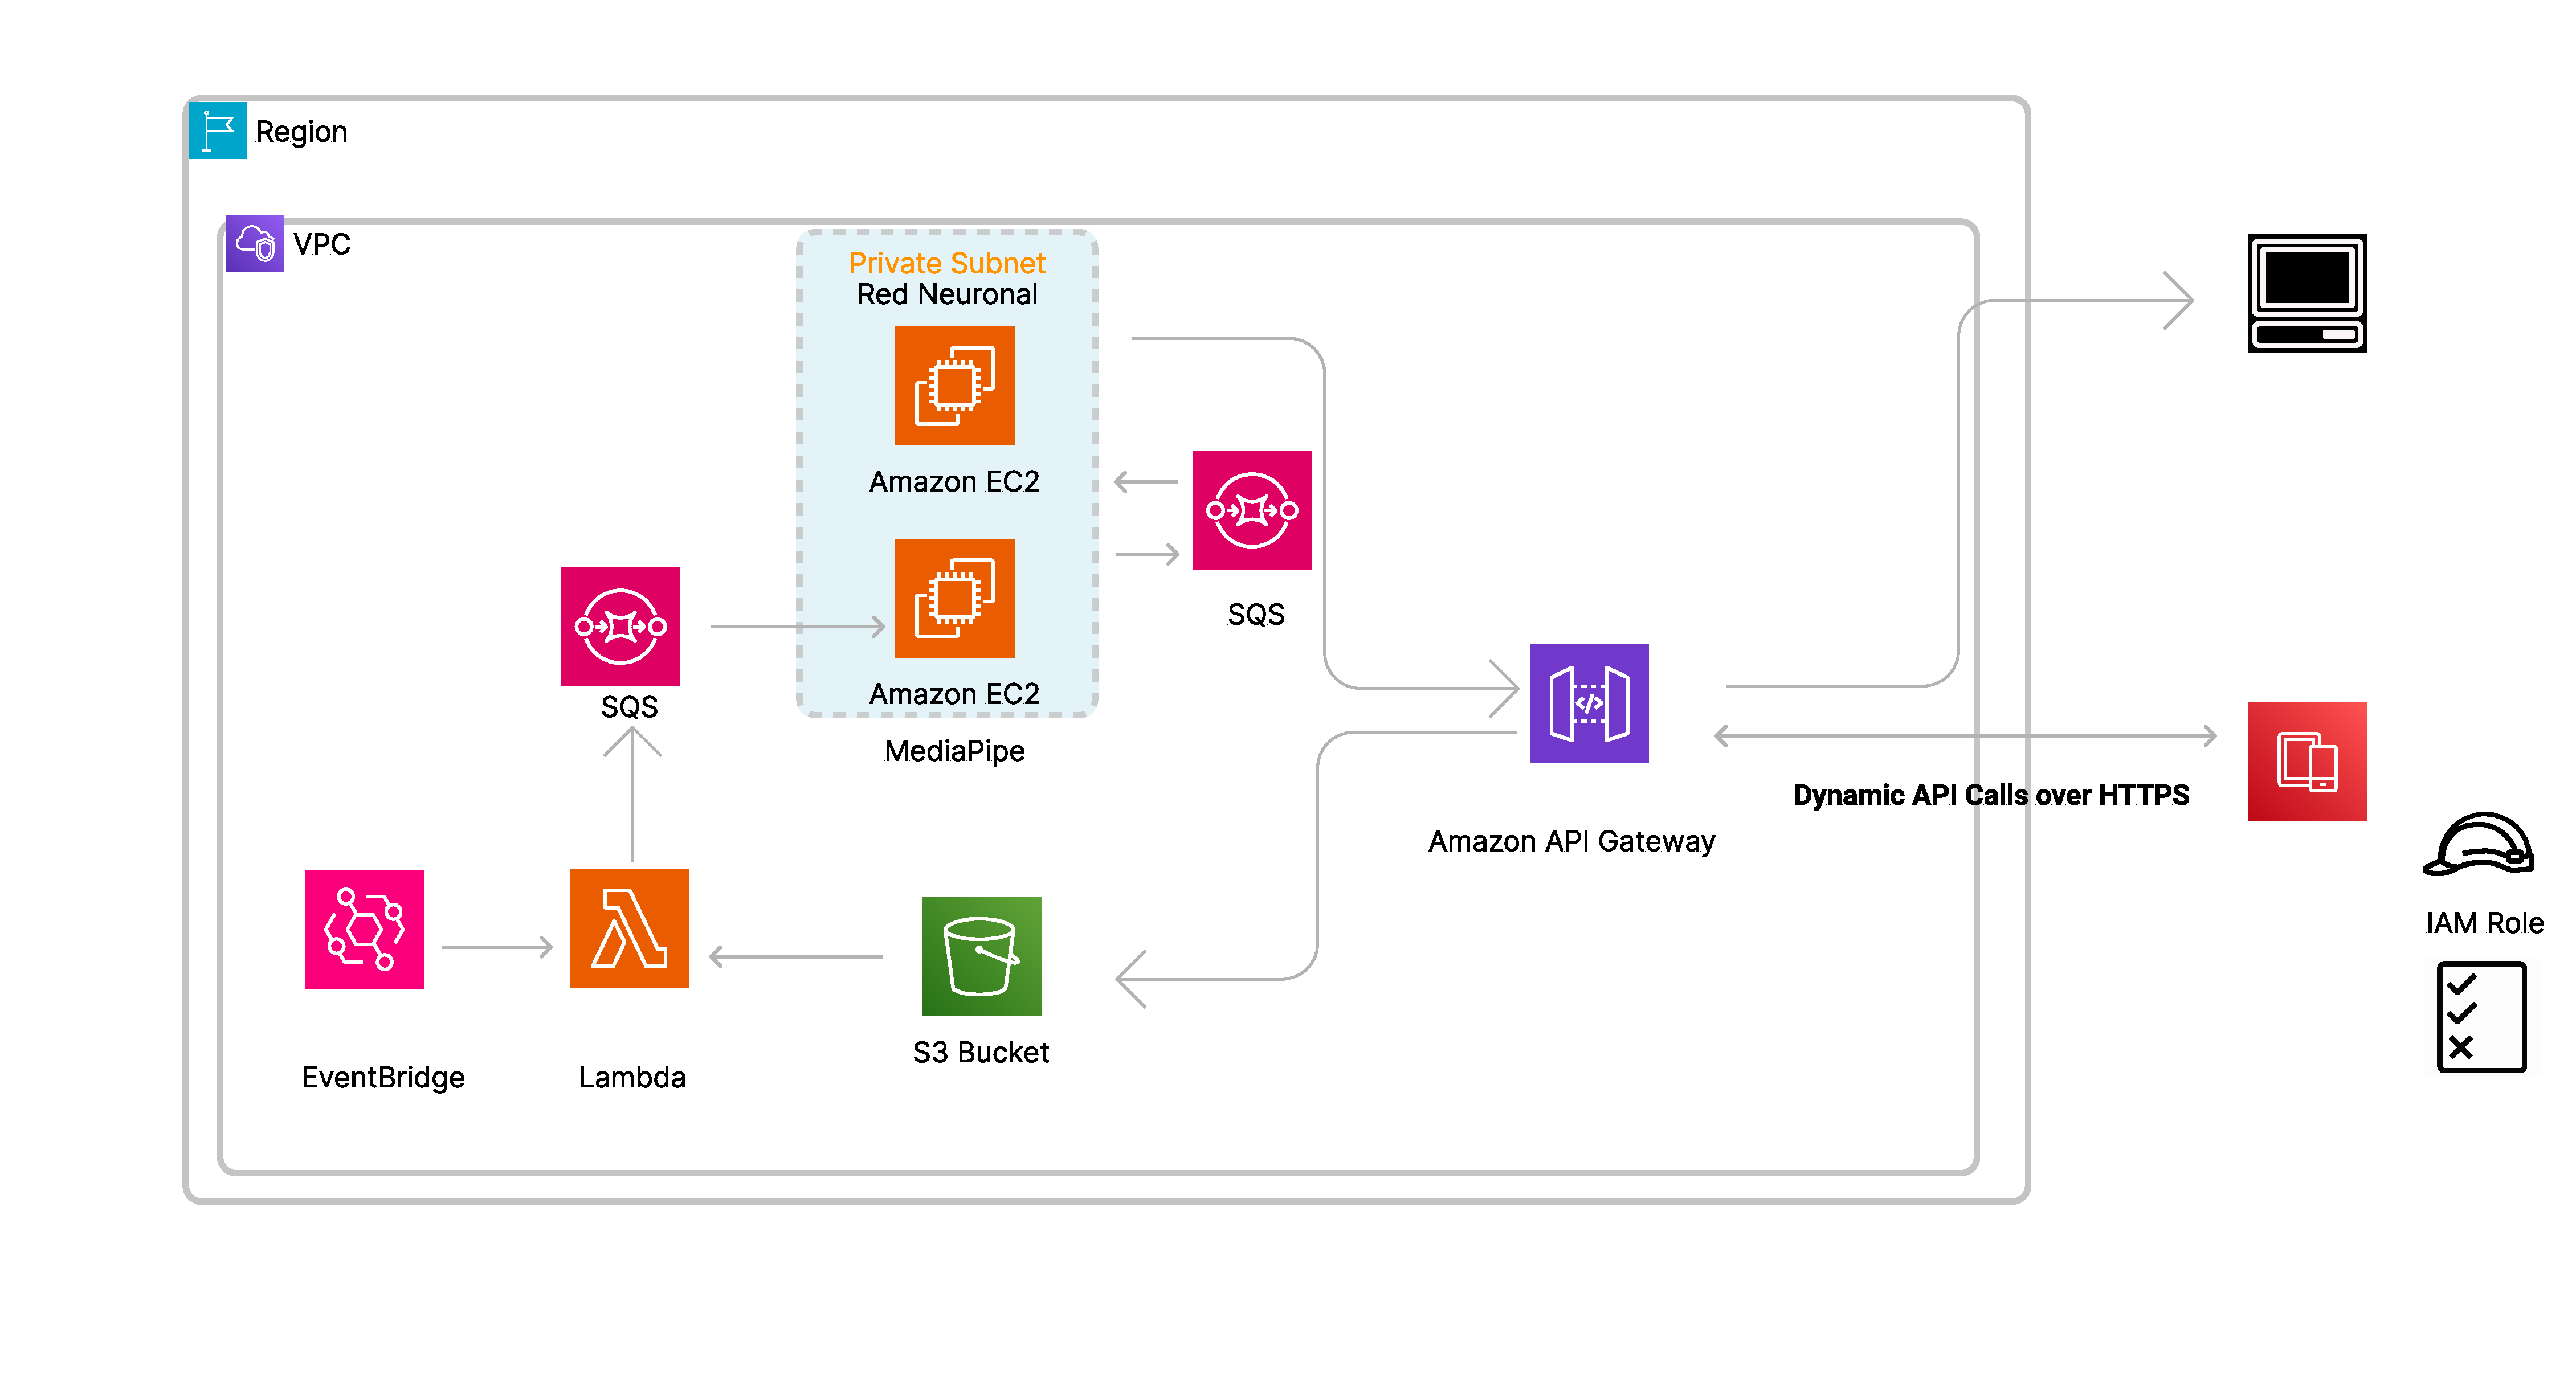
\includegraphics[width=\textwidth]{CAPITULOS/capitulo5/Untitled} % No se incluye la extensión .pdf
\caption{Diagrama de componentes del sistema.}
\label{fig:diagrama_componentes}
\end{figure}
\section{Arquitectura del Sistema}

\begin{itemize}
    \item El programa de obtención de muestreo residirá en un entorno on-premise (en el dispositivo del usuario). Se encargará de capturar los datos, realizar un preprocesamiento básico y enviarlos a la nube.
    \item El sistema de almacenamiento de fotogramas, el entrenamiento del modelo y el despliegue del algoritmo de clasificación se llevarán a cabo en la nube, lo que permitirá escalabilidad y automatización de procesos.
    \item La decisión de desplegar el sistema de traducción en la nube o en un entorno on-premise se basará en un análisis de varios factores, como costo y latencia.
\end{itemize}

\section{Tecnologías Utilizadas}

\begin{itemize}
    \item MediaPipe Holistic (o API similar): Captura y procesamiento de datos de la cámara.
    \item TensorFlow: Entrenamiento y despliegue del modelo de aprendizaje profundo.
    \item Amazon S3: Almacenamiento de fotogramas y datos en la nube.
    \item Python: Lenguaje de programación principal.
    \item API de Text-To-Speech: Generación de mensajes de voz.
    \item Microservicios, SQS, Lambda, EventBridge: Componentes para la arquitectura en la nube (si se opta por esa opción).
    \item Tecnologías web: Sistema web (en conjunto con su framework).
\end{itemize}

\section{Desarrollo de un Sistema de Reconocimiento de Señas}
El sistema de reconocimiento de señas que se desarrollará utilizará principalmente la información de la posición de las falanges de la mano y el antebrazo, capturada a través de una cámara web. Para el seguimiento de manos, se empleará \textbf{MediaPipe Holistic} u otra API de \textbf{hand tracking} que cumpla con criterios de precisión, velocidad, facilidad de integración y soporte para el reconocimiento de la \textbf{Lengua de Señas Mexicana (LSM)}.

Este trabajo se centra en la configuración manual, es decir, en la forma y posición de las manos y los antebrazos durante la realización de una seña. Es importante tener en cuenta que el uso de una cámara implica limitaciones en el campo de visión. Aunque ofrece mayor flexibilidad que algunos sensores, factores como el entorno y la distancia a la cámara pueden afectar la calidad de la captura de datos. Por ello, el sistema se enfocará en la parte superior del cuerpo del usuario, desde los antebrazos hacia arriba, incluyendo las manos, que son las áreas clave para la expresión en LSM.

El flujo de trabajo del sistema, ilustrado en el diagrama \ref{fig:diagrama_composicion}, se desarrolla de la siguiente manera:

\begin{itemize}
    \item \textbf{Iniciar Grabación/Toma de Fotos}: El usuario inicia el proceso, lo que activa la captura de video o fotos.
    \item \textbf{Captura y Procesamiento de Datos}: El sistema divide el video en frames y almacena estos datos localmente antes de subirlos a la nube.
    \item \textbf{Almacenamiento y Notificación}: Los frames se almacenan en un bucket de S3, y se envían notificaciones a través de \textbf{EventBridge}.
    \item \textbf{Invocación de Microservicios}: Se invoca un microservicio que procesa los frames utilizando \textbf{MediaPipe} para extraer características relevantes de las manos y antebrazos.
    \item \textbf{Entrenamiento y Predicción}: Los modelos de machine learning se entrenan con los datos procesados. Cuando el usuario inicia la traducción, el sistema captura frames, predice las palabras en base a un modelo local y genera el audio correspondiente a la seña.
\end{itemize}

El sistema no solo busca reconocer las señas de manera precisa, sino también facilitar la comunicación efectiva mediante la generación de audio en tiempo real, que se reproducirá para el usuario. Además, el enfoque en la parte superior del cuerpo garantiza que se capture adecuadamente la expresión manual esencial para el reconocimiento de la LSM.


\begin{figure}[h]
    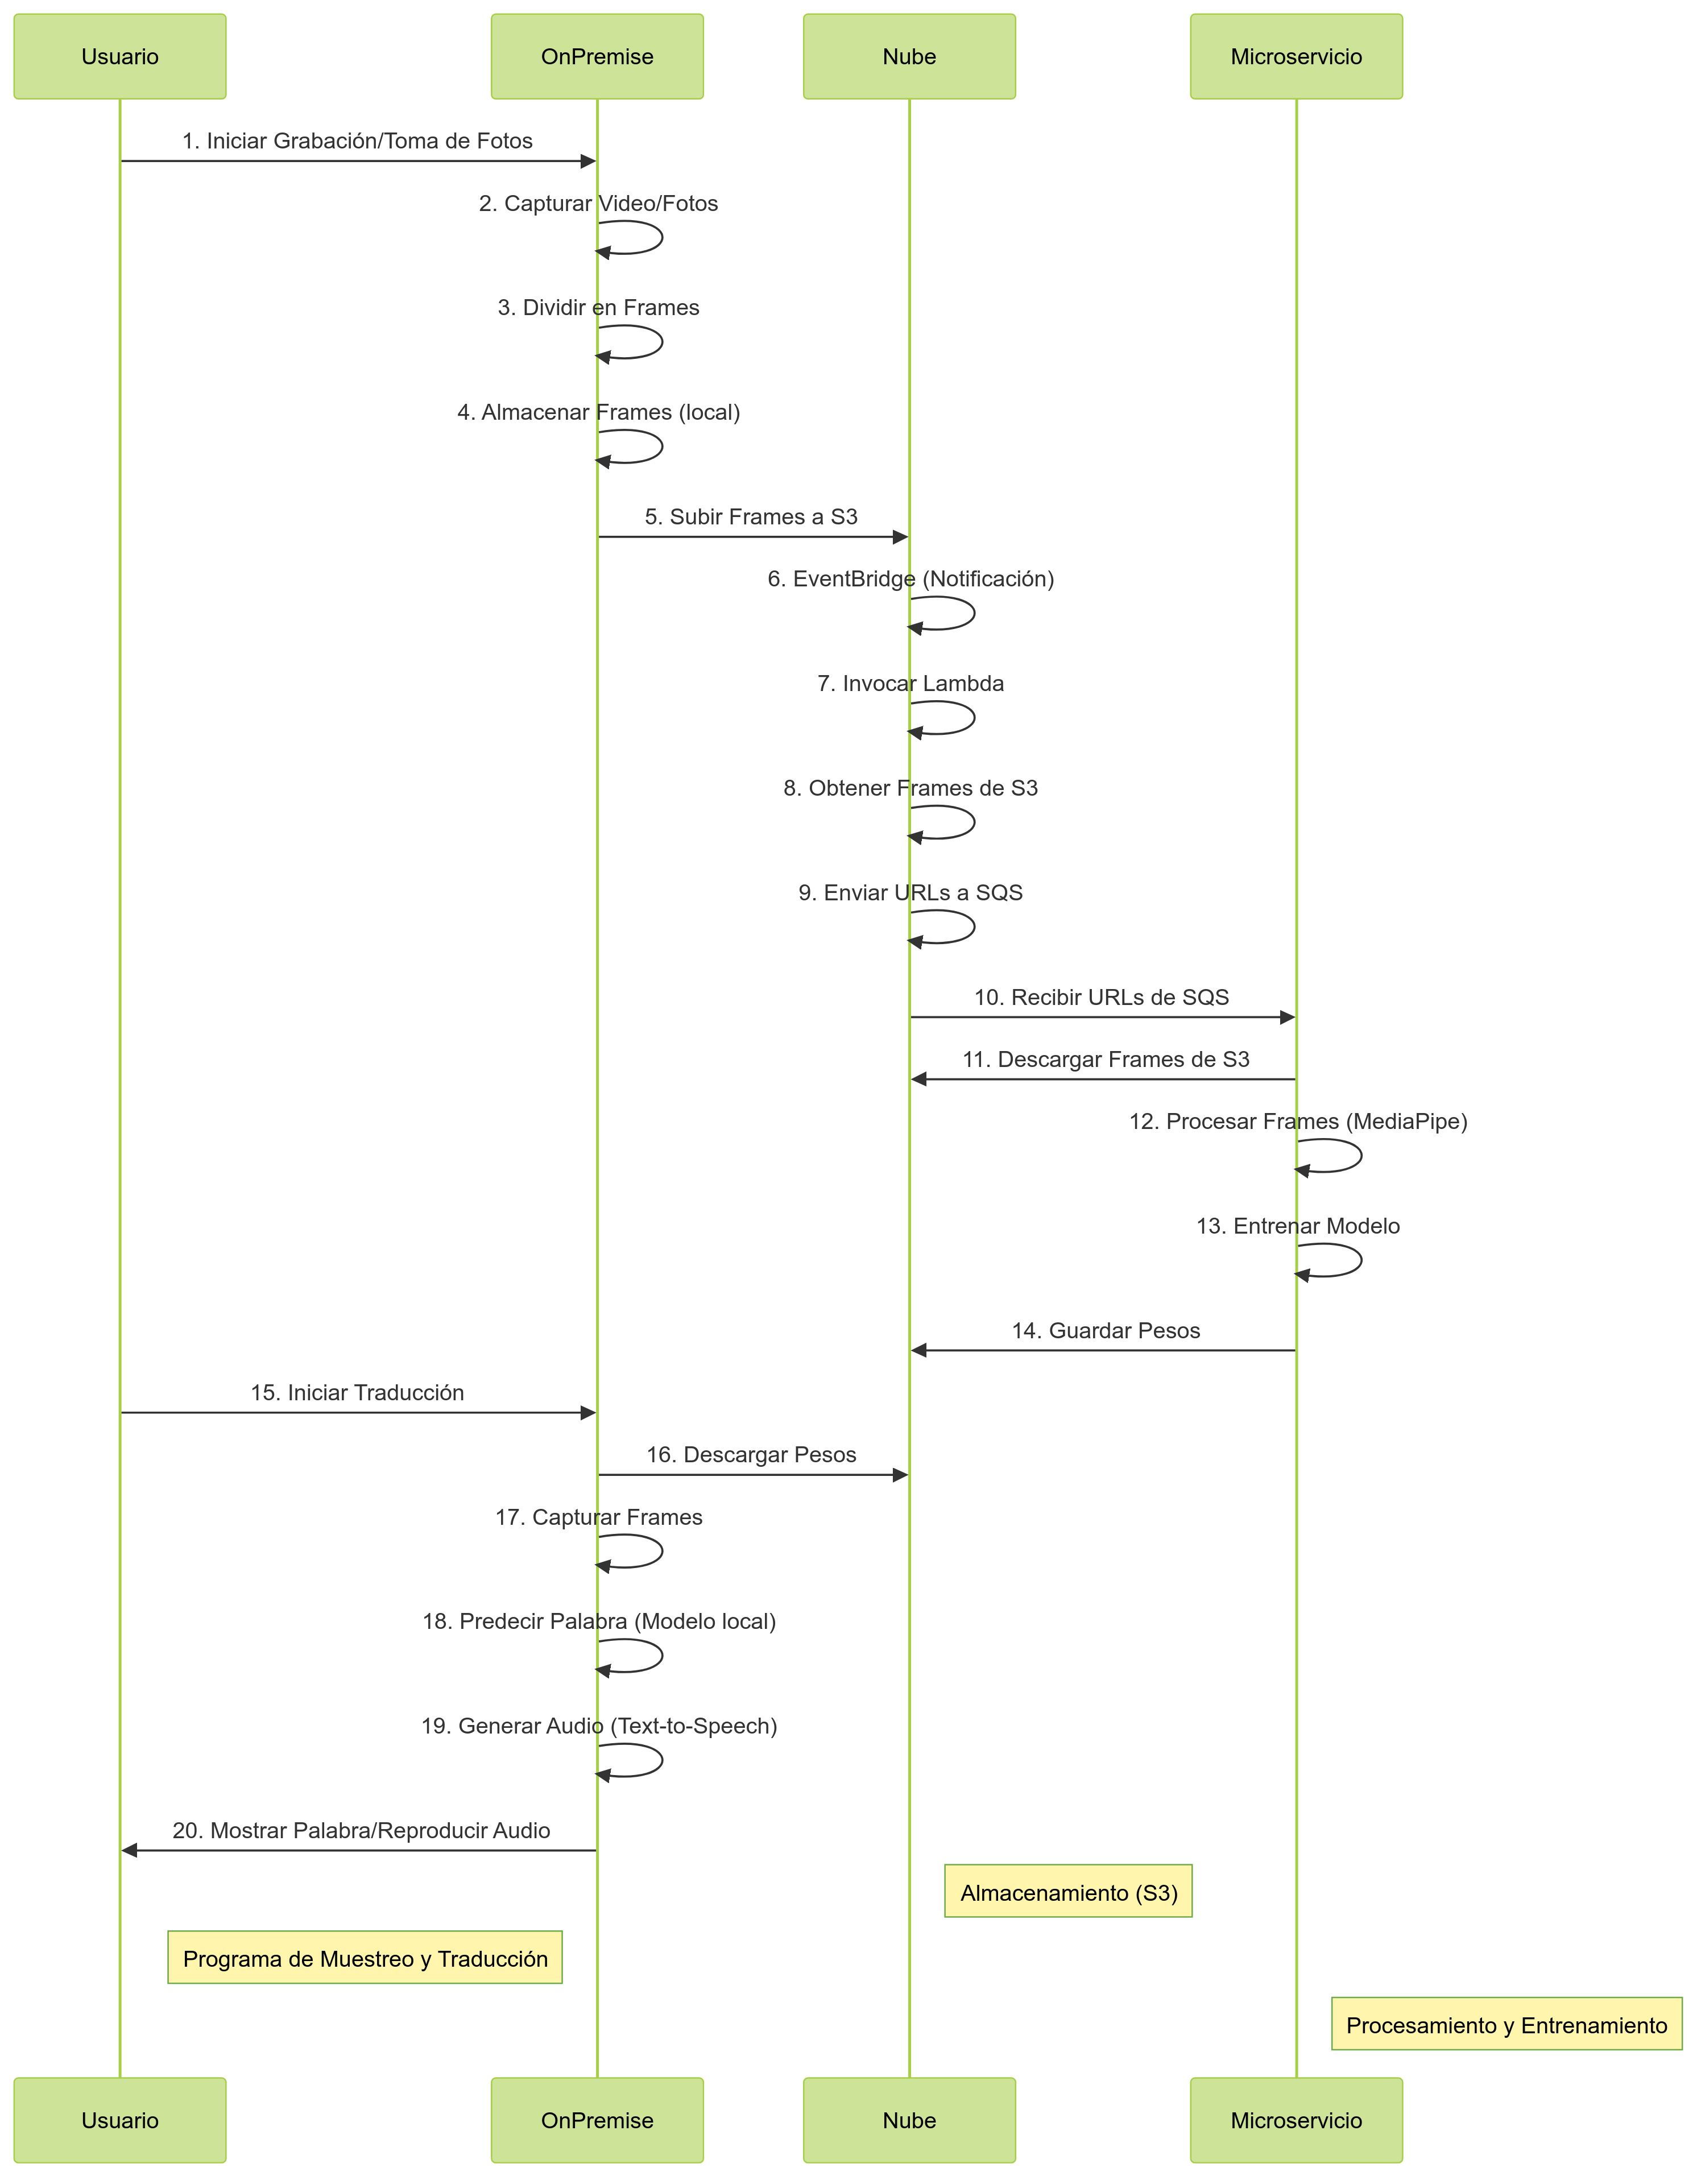
\includegraphics[scale=0.17]{CAPITULOS/capitulo1/segundo.png}
    \centering
    \caption[Diagrama de secuencia composición del sistema ]{Diagrama de secuencia composición del sistema}
    \label{fig:diagrama_composicion}
\end{figure}

\clearpage
\section{Proceso de Muestreo}

El proceso de reconocimiento comenzará cuando el usuario realice un gesto específico de inicio, como alzar la mano. A partir de ese momento, se capturarán fotogramas (frames) de la seña. Estos datos se almacenarán en la nube, utilizando un servicio como Amazon S3, para su posterior procesamiento.

\section{Proceso de Extracción de Datos y Entrenamiento}

La API de MediaPipe Holistic (u otra similar) se encargará de procesar los fotogramas y extraer la posición de los puntos de referencia relevantes en las manos y antebrazos. Una vez que se hayan recopilado suficientes muestras de entrenamiento, se utilizará un microservicio en Python que utilice TensorFlow o Keras para entrenar un modelo de aprendizaje profundo capaz de reconocer las señas. Este modelo se desplegará en la nube para garantizar la escalabilidad y el manejo eficiente de las solicitudes de entrenamiento.

\section{Reconocimiento y Traducción de Señas}

El algoritmo entrenado clasificará la seña emitida, comparándola con las señas previamente clasificadas y entradas. Para ello, utilizará la información de la posición de los puntos de referencia proporcionada por la API de hand tracking y realizará un mapeo a la configuración manual de la seña, como entrada al modelo. Una vez que se logre el reconocimiento de una seña dentro de la LSM, el sistema proporcionará la traducción al español, seguida de un mensaje de voz generado mediante una API de Text-To-Speech.



\section{Base de datos}
\label{sec:base_datos}


Para este módulo se decidió utilizar una base de datos documental (NoSQL).

\subsection{Estructura de las colecciones de Firebase}

A continuación se muestra la estructura de las colecciones de Firebase:

\subsection{Colección usuarios}

\begin{lstlisting}[style=json, caption=Documento de ejemplo en la colección 'usuarios', label=lst:usuarios]
{
  "uid1": {
    "nombre": "jose daniel alvarez ramos",
    "correo": "jalvarezr1001@alumno.ipn.mx",
    "rolId": "admin", // Referencia al documento 'admin' de 'roles'
    "fechaCreacion": "2024-11-09T12:00:00Z",
    "ultimaModificacion": "2024-11-09T12:00:00Z",
    "activo": true,
    "destacados": {
      "conteo": 10,
      "fechaCreacion": "2024-11-09T12:00:00Z",
      "ultimaModificacion": "2024-11-09T12:00:00Z",
      "activo": true
    }
  },
  "uid2": {
    // ... otros usuarios
  }
}
\end{lstlisting}

\subsection{Colección señas}

\begin{lstlisting}[style=json, caption=Documento de ejemplo en la colección 'senas', label=lst:senas]
{
  "sena": {
    "nombre": "Hola",
    "descripcion": "Descripción de la Seña "hola"",
    "videoUrl": "https://bucket.com/hola.mp4",
    "usuarioId": "uid1", // Referencia al documento 'uid1' de 'usuarios'
    "fechaCreacion": "2024-11-09T12:00:00Z",
    "ultimaModificacion": "2024-11-09T12:00:00Z",
    "activo": true
  },
  "sena": {
    // ... otras senas
  }
}
\end{lstlisting}

\subsection{Colección roles}

\begin{lstlisting}[style=json, caption=Documento de ejemplo en la colección 'roles', label=lst:roles]
{
  "admin": {
    "nombre": "Administrador",
    "activo": true
  },
  "usuario": {
    // ... otros roles
  }
}
\end{lstlisting}

\section{Diccionario LSM}
\label{sec:diccionario_LSM}

El \textbf{Diccionario LSM} es un recurso clave en el sistema de traducción, diseñado para almacenar y organizar un extenso repertorio de señas en Lengua de Señas Mexicana (LSM). Este diccionario proporciona las referencias necesarias para el reconocimiento y la correcta traducción de señas, facilitando tanto el aprendizaje de LSM como la interacción entre personas oyentes y personas sordas.

\subsection{Señas y Descripciones}

\begin{itemize}
        % Seña "Bien" con 4 fotogramas
    \item \textbf{Seña: Bien} \\
    La figura a continuación muestra diferentes perspectivas para realizar la seña ``Bien'' en LSM.
    \begin{figure}[H]
        \centering
        \begin{minipage}{0.42\textwidth}
            \centering
            \subfloat[1]{%
                \includegraphics[page=1, width=\textwidth]{CAPITULOS/capitulo5/bien.pdf}
            }
        \end{minipage}%
        \hspace{0.05\textwidth}
        \begin{minipage}{0.42\textwidth}
            \centering
            \subfloat[2]{%
                \includegraphics[page=2, width=\textwidth]{CAPITULOS/capitulo5/bien.pdf}
            }
        \end{minipage}

        \vspace{10pt}

        \begin{minipage}{0.42\textwidth}
            \centering
            \subfloat[3]{%
                \includegraphics[page=3, width=\textwidth]{CAPITULOS/capitulo5/bien.pdf}
            }
        \end{minipage}%
        \hspace{0.05\textwidth}
        \begin{minipage}{0.42\textwidth}
            \centering
            \subfloat[4]{%
                \includegraphics[page=4, width=\textwidth]{CAPITULOS/capitulo5/bien.pdf}
            }
        \end{minipage}

        \caption{Composición de la Seña ``Bien'' en LSM}
        \label{fig:seña_bien}
    \end{figure}

    % Seña "Hola" con 3 fotogramas
    \item \textbf{Seña: Hola} \\
    \begin{figure}[H]
        \centering
        \begin{minipage}{0.42\textwidth}
            \centering
            \subfloat[1]{%
                \includegraphics[page=1, width=\textwidth]{CAPITULOS/capitulo5/hola.pdf}
            }
        \end{minipage}%
        \hspace{0.05\textwidth}
        \begin{minipage}{0.42\textwidth}
            \centering
            \subfloat[2]{%
                \includegraphics[page=2, width=\textwidth]{CAPITULOS/capitulo5/hola.pdf}
            }
        \end{minipage}

        \vspace{10pt}

        \begin{minipage}{0.45\textwidth}
            \centering
            \subfloat[3]{%
                \includegraphics[page=3, width=\textwidth]{CAPITULOS/capitulo5/hola.pdf}
            }
        \end{minipage}

        \caption{Composición de la Seña ``Hola'' en LSM}
        \label{fig:seña_hola}
    \end{figure}

    % Seña "Mal" con 4 fotogramas
    \item \textbf{Seña: Mal} \\
    \begin{figure}[H]
        \centering
        \begin{minipage}{0.42\textwidth}
            \centering
            \subfloat[1]{%
                \includegraphics[page=1, width=\textwidth]{CAPITULOS/capitulo5/mal.pdf}
            }
        \end{minipage}%
        \hspace{0.05\textwidth}
        \begin{minipage}{0.42\textwidth}
            \centering
            \subfloat[2]{%
                \includegraphics[page=2, width=\textwidth]{CAPITULOS/capitulo5/mal.pdf}
            }
        \end{minipage}

        \vspace{10pt}

        \begin{minipage}{0.45\textwidth}
            \centering
            \subfloat[3]{%
                \includegraphics[page=3, width=\textwidth]{CAPITULOS/capitulo5/mal.pdf}
            }
        \end{minipage}%
        \hspace{0.05\textwidth}
        \begin{minipage}{0.45\textwidth}
            \centering
            \subfloat[4]{%
                \includegraphics[page=4, width=\textwidth]{CAPITULOS/capitulo5/mal.pdf}
            }
        \end{minipage}

        \caption{Composición de la Seña ``Mal'' en LSM}
        \label{fig:seña_mal}
    \end{figure}

    % Seña "¿Cómo estás?" con 5 fotogramas
    \item \textbf{Seña: ¿Cómo estás?} \\
    \begin{figure}[H]
        \centering
        \begin{minipage}{0.28\textwidth}
            \centering
            \subfloat[1]{%
                \includegraphics[page=1, width=\textwidth]{CAPITULOS/capitulo5/como.pdf}
            }
        \end{minipage}%
        \hspace{0.05\textwidth}
        \begin{minipage}{0.28\textwidth}
            \centering
            \subfloat[2]{%
                \includegraphics[page=2, width=\textwidth]{CAPITULOS/capitulo5/como.pdf}
            }
        \end{minipage}

        \vspace{10pt}

        \begin{minipage}{0.28\textwidth}
            \centering
            \subfloat[3]{%
                \includegraphics[page=3, width=\textwidth]{CAPITULOS/capitulo5/como.pdf}
            }
        \end{minipage}%
        \hspace{0.05\textwidth}
        \begin{minipage}{0.28\textwidth}
            \centering
            \subfloat[4]{%
                \includegraphics[page=4, width=\textwidth]{CAPITULOS/capitulo5/como.pdf}
            }
        \end{minipage}

        \vspace{10pt}

        \begin{minipage}{0.3\textwidth}
            \centering
            \subfloat[5]{%
                \includegraphics[page=5, width=\textwidth]{CAPITULOS/capitulo5/como.pdf}
            }
        \end{minipage}

        \caption{Composición de la Seña ``¿Cómo estás?'' en LSM}
        \label{fig:seña_como_estas}
    \end{figure}

    \item \textbf{Seña: Doctor} \\
    \begin{figure}[H]
        \centering
        \begin{minipage}{0.42\textwidth}
            \centering
            \subfloat[1]{%
                \includegraphics[page=1, width=\textwidth]{CAPITULOS/capitulo5/doctor}
            }
        \end{minipage}%
        \hspace{0.05\textwidth}
        \begin{minipage}{0.42\textwidth}
            \centering
            \subfloat[2]{%
                \includegraphics[page=2, width=\textwidth]{CAPITULOS/capitulo5/doctor}
            }
        \end{minipage}

        \vspace{10pt}

        \begin{minipage}{0.45\textwidth}
            \centering
            \subfloat[3]{%
                \includegraphics[page=3, width=\textwidth]{CAPITULOS/capitulo5/doctor}
            }
        \end{minipage}

        \caption{Composición de la Seña ``Doctor'' en LSM}
        \label{fig:seña_doctor}
    \end{figure}

    % Seña "Mal" con 4 fotogramas
    \item \textbf{Seña: Emergencia} \\
    \begin{figure}[H]
        \centering
        \begin{minipage}{0.42\textwidth}
            \centering
            \subfloat[1]{%
                \includegraphics[page=1, width=\textwidth]{CAPITULOS/capitulo5/emergencia}
            }
        \end{minipage}%
        \hspace{0.05\textwidth}
        \begin{minipage}{0.42\textwidth}
            \centering
            \subfloat[2]{%
                \includegraphics[page=2, width=\textwidth]{CAPITULOS/capitulo5/emergencia}
            }
        \end{minipage}

        \vspace{10pt}

        \begin{minipage}{0.45\textwidth}
            \centering
            \subfloat[3]{%
                \includegraphics[page=3, width=\textwidth]{CAPITULOS/capitulo5/emergencia}
            }
        \end{minipage}%
        \hspace{0.05\textwidth}
        \begin{minipage}{0.45\textwidth}
            \centering
            \subfloat[4]{%
                \includegraphics[page=4, width=\textwidth]{CAPITULOS/capitulo5/emergencia}
            }
        \end{minipage}

        \caption{Composición de la Seña ``Emergencia'' en LSM}
        \label{fig:seña_emergencia}
    \end{figure}

    % Seña "Hola" con 3 fotogramas
    \item \textbf{Seña: Por favor} \\
    \begin{figure}[H]
        \centering
        \begin{minipage}{0.42\textwidth}
            \centering
            \subfloat[1]{%
                \includegraphics[page=1, width=\textwidth]{CAPITULOS/capitulo5/porfavor}
            }
        \end{minipage}%
        \hspace{0.05\textwidth}
        \begin{minipage}{0.42\textwidth}
            \centering
            \subfloat[2]{%
                \includegraphics[page=2, width=\textwidth]{CAPITULOS/capitulo5/porfavor}
            }
        \end{minipage}

        \vspace{10pt}

        \begin{minipage}{0.45\textwidth}
            \centering
            \subfloat[3]{%
                \includegraphics[page=3, width=\textwidth]{CAPITULOS/capitulo5/porfavor}
            }
        \end{minipage}

        \caption{Composición de la Seña ``Por favor'' en LSM}
        \label{fig:seña_porfavor}
    \end{figure}

    % Seña "Mal" con 4 fotogramas
    \item \textbf{Seña: Síntoma} \\
    \begin{figure}[H]
        \centering
        \begin{minipage}{0.42\textwidth}
            \centering
            \subfloat[1]{%
                \includegraphics[page=1, width=\textwidth]{CAPITULOS/capitulo5/sintoma}
            }
        \end{minipage}%
        \hspace{0.05\textwidth}
        \begin{minipage}{0.42\textwidth}
            \centering
            \subfloat[2]{%
                \includegraphics[page=2, width=\textwidth]{CAPITULOS/capitulo5/sintoma}
            }
        \end{minipage}

        \vspace{10pt}

        \begin{minipage}{0.45\textwidth}
            \centering
            \subfloat[3]{%
                \includegraphics[page=3, width=\textwidth]{CAPITULOS/capitulo5/sintoma}
            }
        \end{minipage}%
        \hspace{0.05\textwidth}
        \begin{minipage}{0.45\textwidth}
            \centering
            \subfloat[4]{%
                \includegraphics[page=4, width=\textwidth]{CAPITULOS/capitulo5/sintoma}
            }
        \end{minipage}

        \caption{Composición de la Seña ``Síntoma'' en LSM}
        \label{fig:seña_sintoma}
    \end{figure}

    \item \textbf{Seña: Temperatura} \\
    \begin{figure}[H]
        \centering
        \begin{minipage}{0.42\textwidth}
            \centering
            \subfloat[1]{%
                \includegraphics[page=1, width=\textwidth]{CAPITULOS/capitulo5/temperatura}
            }
        \end{minipage}%
        \hspace{0.05\textwidth}
        \begin{minipage}{0.42\textwidth}
            \centering
            \subfloat[2]{%
                \includegraphics[page=2, width=\textwidth]{CAPITULOS/capitulo5/temperatura}
            }
        \end{minipage}

        \vspace{10pt}

        \begin{minipage}{0.45\textwidth}
            \centering
            \subfloat[3]{%
                \includegraphics[page=3, width=\textwidth]{CAPITULOS/capitulo5/temperatura}
            }
        \end{minipage}%
        \hspace{0.05\textwidth}
        \begin{minipage}{0.45\textwidth}
            \centering
            \subfloat[4]{%
                \includegraphics[page=4, width=\textwidth]{CAPITULOS/capitulo5/temperatura}
            }
        \end{minipage}

        \caption{Composición de la Seña ``Temperatura'' en LSM}
        \label{fig:seña_temperatura}
    \end{figure}

    \item \textbf{Seña: Enfermo} \\
    \begin{figure}[H]
        \centering
        \begin{minipage}{0.42\textwidth}
            \centering
            \subfloat[1]{%
                \includegraphics[page=1, width=\textwidth]{CAPITULOS/capitulo5/enfermo}
            }
        \end{minipage}%
        \hspace{0.05\textwidth}
        \begin{minipage}{0.42\textwidth}
            \centering
            \subfloat[2]{%
                \includegraphics[page=2, width=\textwidth]{CAPITULOS/capitulo5/enfermo}
            }
        \end{minipage}

        \vspace{10pt}

        \begin{minipage}{0.45\textwidth}
            \centering
            \subfloat[3]{%
                \includegraphics[page=3, width=\textwidth]{CAPITULOS/capitulo5/enfermo}
            }
        \end{minipage}%
        \hspace{0.05\textwidth}
        \begin{minipage}{0.45\textwidth}
            \centering
            \subfloat[4]{%
                \includegraphics[page=4, width=\textwidth]{CAPITULOS/capitulo5/enfermo}
            }
        \end{minipage}

        \caption{Composición de la Seña ``Enfermo'' en LSM}
        \label{fig:seña_enfermo}
    \end{figure}
\end{itemize}

\section{Interfaz de usuario de la aplicación}

La aplicación móvil se ha diseñado con una interfaz intuitiva y fácil de usar, con el objetivo de proporcionar una experiencia de usuario fluida y accesible. A continuación, se describen las principales pantallas de la aplicación, diferenciando entre los roles de usuario (administrador y general) cuando sea necesario:

\subsection{Splash Screen}

\begin{figure}[h]
    \centering
    \fbox{\includegraphics[page=1, scale=0.5]{CAPITULOS/capitulo5/proyecto}}
    \caption{Splash Screen de la aplicación.}
\end{figure}

Esta es la primera pantalla que se muestra al iniciar la aplicación. Su función principal es mostrar el ícono de la aplicación mientras se cargan los componentes necesarios.  Es visible tanto para usuarios administradores como generales.

\subsection{Login}

\begin{figure}[h]
    \centering
    \fbox{\includegraphics[page=2, scale=0.5]{CAPITULOS/capitulo5/proyecto}}
    \caption{Pantalla de inicio de sesión.}
\end{figure}

Esta pantalla permite a todos los usuarios iniciar sesión en la aplicación. Se requiere una dirección de correo electrónico y una contraseña para la autenticación, la cual se gestiona a través de Firebase.

\subsubsection{Funcionalidad}

\begin{itemize}
    \item \textbf{Inicio de sesión con correo electrónico y contraseña:} Disponible para todos los usuarios.
    \item \textbf{Inicio de sesión con Google:} Disponible solo para usuarios con rol general.
    \item \textbf{Registro de nuevo usuario:} Permite a los usuarios que no están registrados crear una cuenta utilizando su correo electrónico y contraseña, o a través de su cuenta de Google.
\end{itemize}
\subsection{Pantalla principal (Usuario general)}

\begin{figure}[h]
    \centering
    \fbox{\includegraphics[page=3, scale=0.5]{CAPITULOS/capitulo5/proyecto}}
    \caption{Pantalla principal para usuarios con rol general.}
\end{figure}

Esta es la pantalla principal a la que acceden los usuarios con rol general después de iniciar sesión.

\subsubsection{Diseño}

El diseño de la pantalla principal es simple y directo. En la parte superior se encuentra el logo de la aplicación, y en la parte central se muestran las opciones principales, como "Traducir" y "Diccionario". Cada opción se representa con un icono y un texto descriptivo.

\subsubsection{Funcionalidad}

Al tocar una de las opciones, el usuario es redirigido a la pantalla correspondiente. Por ejemplo, al tocar "Traducir", se abre la pantalla de traducción en tiempo real.

\subsection{Pantalla principal (Usuario administrador)}

\begin{figure}[h]
    \centering
    \fbox{\includegraphics[page=4, scale=0.5]{CAPITULOS/capitulo5/proyecto}}
    \caption{Pantalla principal para usuarios administradores.}
\end{figure}

Esta es la pantalla principal a la que acceden los usuarios administradores después de iniciar sesión.

[Aquí deberías describir el diseño y la funcionalidad específica de la pantalla principal para el usuario administrador, incluyendo las opciones adicionales a las que tiene acceso, como la gestión de usuarios, la edición del diccionario, etc.]

\subsection{Pantalla del diccionario}

\begin{figure}[h]
    \centering
    \fbox{\includegraphics[page=5, scale=0.5]{CAPITULOS/capitulo5/proyecto}}
    \caption{Pantalla del diccionario LSM.}
\end{figure}

[El resto de la descripción de la pantalla del diccionario se mantiene igual]



